\subsection*{Fatorações de polinômios}

Quando temos expressões polinomiais, é importante saber como fatorá-las.

\begin{itemize}
	\item $x^2-y^2=(x-y)(x+y)$
	\item $x^3-y^3=(x-y)(x^2+xy+y^2)$
	\item $x^4-y^4=(x-y)(x^3+x^2y+xy^2+y^3$
	\item $x^n-y^n=(x-y)(x^{n-1}+x^{n-2}y+x^{n-3}y^2+\cdots+x^2y^{n-3}+xy^{n-2}+y^{n-1})$
	\item Se $n$ é ímpar, então $x^n+y^n=(x+y)(x^{n-1}-x^{n-2}y+x^{n-3}y^2+\cdots+x^2y^{n-3}-xy^{n-2}+y^{n-1})$ (note que os sinais do segundo termo se alternam).
\end{itemize}

É possível usar as fatorações acima com raízes, por meio de uma \emph{mudança de variáveis}: Sejam $z=x^n$ e $w=y^n$. Então a quarta fórmula acima pode ser reescrita como
\[z-w=(\sqrt[n]{z}-\sqrt[n]{w})(\sqrt[n]{z^{n-1}}+\sqrt[n]{z^{n-2}w}+\cdots+\sqrt[n]{zw^{n-2}}+\sqrt[n]{w^{n-1}})\]

\subsection*{Fórmulas trigonométricas}

Um dos jeitos mais fáceis de se lembrar como seno e cosseno são definidos é usando o \emph{círculo trigonométrico}:

\[\begin{tikzpicture}
	\draw[latex-latex] (-3,0)--(3,0) ; %x axis
	\draw[latex-latex] (0,-3)--(0,3) ; %y axis
	
	\draw (0,0) circle (2);
    \draw[thick,blue,dashed] (.5,0) arc (0:50:.5) node[midway,right] {$x$};
    \draw[thick,blue] (2,0) arc (0:50:2);
    
    \draw[thick,blue] (0,0)--(50:2);
    
    \draw[dashed,blue] (0,1.5320888862379560704047853011)--(50:2)--(1.285575219373078652645286819814526865,0);
    
    \node[below,blue] at (1.285575219373078652645286819814526865,0) {$\cos(x)$};
    
    \node[left, blue] at (0,1.5320888862379560704047853011) {$\sin(x)$};
    
    \node[below left] at (-2,0) {$-\pi$};
    \node[below right] at (2,0) {$0\cong2\pi$};
    \node[above right] at (0,2) {$\dfrac{\pi}{2}$};
    \node[below right] at (0,-2) {$\dfrac{3\pi}{2}$};
\end{tikzpicture}\]

Este é um círculo de centro $(0,0)$ e raio $1$. Um ângulo $x$ é desenhado partindo do ponto $(1,0)$ no sentido anti-horário. Uma volta completa ao redor do círculo corresponde a um ângulo de $2\pi$. O eixo vertical correspondo ao seno $\sin(x)$ do ângulo, e o eixo horizontal corresponde ao cosseno $\cos(x)$.

Simplesmente olhando para o círculo, obtemos

\begin{itemize}
	\item $\sin(0)=0$.
	\item $\sin\left(\dfrac{\pi}{2}\right)=1$.
	\item $\sin(\pi)=0$.
	\item $\sin\left(\dfrac{3\pi}{2}\right)=-1$.
	\item $\cos(0)=1$.
	\item $\cos\left(\dfrac{\pi}{2}\right)=0$.
	\item $\cos(\pi)=-1$.
	\item $\cos\left(\dfrac{3\pi}{2}\right)=0$.
\end{itemize}

e também que
\begin{itemize}
	\item $\sin(-x)=-\sin(x)$.
	\item $\cos(-x)=\cos(x)$.
\end{itemize}

Pelo Teorema de Pitágoras, obtemos
\begin{itemize}
	\item $\sin^2(x)+\cos^2(x)=1$.
\end{itemize}

Tangente e cotangente são definidas do seguinte modo:
\begin{itemize}
	\item $\tan(x)=\dfrac{\sin(x)}{\cos(x)}$, sempre que $\cos(x)\neq 0$.
	\item $\arctan(x)=\dfrac{\cos(x)}{\sin(x)}$, sempre que $\sin(x)\neq 0$.
\end{itemize}

O ângulo de somas e difereças são relacionados por
\end{itemize}
	\item $\sin(x+y)=\sin(x)\cos(y)+\sin(y)\cos(x)$.
	\item $\cos(x+y)=\cos(x)\cos(y)-\sin(x)\sin(y)$.
\end{itemize}

Essencialmente todas as outras fórmulas trigonométricas podem ser obtidas utilizando somente estas fórmulas ``básicas''. Por exemplo, temos que 
\begin{align*}
	\sin\left(\dfrac{\pi}{2}-x\right)&=\sin\left(\dfrac{\pi}{2}\right)\cos(x)-\sin(x)\cos\left(\dfrac{\pi}{2}\right)\\
	&=\cos(x)
\end{align*}

As funções inversas das funções trigonométricas são definidas conforme:
\begin{itemize}
	\item A função $\sin(x)$ é bijetiva no intervalo $\left[-\dfrac{\pi}{2},\dfrac{\pi}{2}\right]$, e $\arcsin(x)$ é a inversa de $\sin(x)$ neste intervalo.
	\item A função $\cos(x)$ é bijetiva no intervalo $\left[0,\pi\right]$, e $\arccos(x)$ é a inversa de $\cos(x)$ neste intervalo.
	\item A função $\tan(x)$ é bijetiva no intervalo $\left(-\dfrac{\pi}{2},\dfrac{\pi}{2}\right)$, e $\arctan(x)$ é a inversa de $\tan(x)$ neste intervalo.
\end{itemize}